\chapter{Uvod}
\label{ch:introduction_background}

\selectlanguage{croatian}

\section{Problemski okvir i motivacija}

U suvremenom digitalnom ekosustavu, otvoreni podaci predstavljaju fundamentalni resurs za unapređenje transparentnosti javne uprave, poticanje znanstvenih istraživanja i generiranje ekonomskih inovacija. Portali poput službenog EU Portala otvorenih podataka nude pristup milijunima skupova podataka koji obuhvaćaju širok spektar domena, od okoliša i energetike do zdravstva i ekonomije. Unatoč golemom intrinzičkom potencijalu, stvarna iskoristivost ovih resursa ostaje na relativno niskoj razini. Uzroci ovog nesrazmjera su višestruki i složeni.

Primarno, postoji tehnička barijera. Pretraživanje i dohvaćanje podataka s portala koji primjenjuju tehnologije semantičkog weba zahtijeva ovladavanje specifičnim upitnim jezicima, među kojima se ističe SPARQL. Navedeni jezik, unatoč svojoj izražajnoj moći, nije intuitivan za korisnike bez formalne tehničke naobrazbe, kao što su novinari, analitičari javnih politika ili studenti. Time se sužava krug potencijalnih korisnika otvorenih podataka.

Nadalje, uočava se nepreciznost tradicionalnih metoda pretrage. Većina postojećih portala implementira pretragu temeljenu na podudaranju ključnih riječi. Takav pristup često rezultira nerelevantnim ishodima jer ne posjeduje sposobnost razumijevanja semantičkog konteksta korisničkog upita. Primjerice, upit "utjecaj prometa na kvalitetu zraka u urbanim sredinama" može propustiti relevantne skupove podataka koji koriste semantički ekvivalentne termine poput "emisije ispušnih plinova vozila" ili "onečišćenje zraka u gradskim područjima".

Posebno značajan izazov predstavlja problem složenih analitičkih pitanja čiji odgovor zahtijeva korištenje i povezivanje više različitih skupova podataka. Najveća vrijednost otvorenih podataka manifestira se upravo kroz njihovu sintezu i međusobno povezivanje s ciljem stjecanja novih spoznaja. Odgovor na složenije analitičko pitanje, kao što je "Analiza korelacije između poljoprivrednih subvencija u NUTS 2 regijama i rasta BDP-a tih regija u posljednjih pet godina", nalaže pronalaženje, interpretaciju i integraciju višestrukih, često heterogenih skupova podataka. Takvi složeni upiti zahtijevaju ne samo identifikaciju relevantnih skupova podataka već i razumijevanje njihovih međusobnih veza, kompatibilnosti formata te mogućnosti integracije. Manualno izvođenje ovog procesa je zahtjevno, vremenski intenzivno i podložno pogreškama.

Dodatno, korisnici se susreću s problemom interpretacije metapodataka. Čak i kada uspiju pronaći potencijalno relevantne skupove podataka, razumijevanje njihove strukture, kvalitete i prikladnosti za specifičnu analizu predstavlja izazov. DCAT standard, iako pruža strukturiran način opisivanja podataka, često zahtijeva tehničko znanje za pravilnu interpretaciju.

Navedeni problemi generiraju diskrepanciju između proklamiranog potencijala otvorenih podataka i njihove stvarne primjene u praksi. Ova diskrepancija čini središnju motivaciju ovog istraživanja.

\section{Predloženo rješenje i ciljevi rada}

S ciljem premošćivanja identificiranog jaza između dostupnosti i iskoristivosti otvorenih podataka, ovaj rad predlaže razvoj inteligentnog sustava za analizu metapodataka otvorenih skupova podataka. Jezgru predloženog rješenja čini arhitektura \textit{Retrieval-Augmented Generation} (RAG)~\cite{lewis2020retrieval}, koja sinergijski kombinira sposobnosti velikih jezičnih modela (LLM) s preciznošću dohvata informacija iz strukturiranih baza znanja.

Sustav je projektiran s namjerom da korisnički upit, formuliran na prirodnom jeziku, prevede u sintaksno ispravan i semantički relevantan SPARQL upit. Ova transformacija omogućava premošćivanje jaza između intuitivnog načina na koji korisnici postavljaju pitanja i formalnog jezika potrebnog za interakciju s bazama podataka semantičkog weba.

Operativni proces sustava započinje pretraživanjem interne vektorske baze podataka radi pronalaska relevantnih primjera prethodno formuliranih upita i informacija o strukturi (shemi) podataka dostupnih na portalu. Vektorska baza koristi tehnike semantičkog pretraživanja temeljene na \textit{embeddings} tehnologiji, što omogućava pronalaženje sličnih upita čak i kada ne postoji doslovno podudaranje ključnih riječi. Dohvaćene informacije, koje čine kontekst, pridružuju se originalnom korisničkom upitu. Tako obogaćen unos prosljeđuje se velikom jezičnom modelu (npr. GPT-4)~\cite{brown2020language}, koji na temelju pruženog konteksta generira ciljani SPARQL upit.

Glavni cilj rada jest implementacija i evaluacija funkcionalnog prototipa opisanog sustava, s primjenom na EU Portal otvorenih podataka. Specifični ciljevi rada obuhvaćaju:

\begin{enumerate}
    \item \textbf{Dizajnirati i implementirati RAG arhitekturu} optimiziranu za generiranje SPARQL upita. Ova arhitektura mora biti sposobna kombinirati prednosti semantičkog pretraživanja s generativnim sposobnostima velikih jezičnih modela.
    
    \item \textbf{Uspostaviti i održavati vektorsku bazu podataka} koja sadrži reprezentativne primjere upita i relevantne metapodatke o shemi. Baza mora biti strukturirana na način koji omogućava brzo i precizno dohvaćanje relevantnih informacija.
    
    \item \textbf{Implementirati multimodalni pristup pretraživanju} koji integrira RAG-generirane SPARQL upite, REST API pozive i pretragu po sličnosti. Ovaj hibridni pristup osigurava stabilnost sustava i pokriva različite scenarije korištenja.
    
    \item \textbf{Razviti mehanizme za rukovanje složenim upitima} koji zahtijevaju podatke iz više različitih skupova. Sustav mora biti sposoban identificirati potrebu za integracijom podataka i predložiti strategije za njihovo povezivanje.
    
    \item \textbf{Sustavno evaluirati performanse, točnost i stabilnost} razvijenog prototipa kroz sveobuhvatan skup testnih scenarija koji pokrivaju različite domene i razine složenosti.
    
    \item \textbf{Pružiti detaljan inženjerski nacrt} rješenja koje je modularno, transparentno i pogodno za daljnju nadogradnju. Dokumentacija mora omogućiti drugim istraživačima i praktičarima reproduciranje i proširivanje sustava.
\end{enumerate}

Krajnji ishod ovog rada je sustav koji pridonosi demokratizaciji pristupa otvorenim podacima, omogućujući korisnicima bez specijaliziranih tehničkih znanja postavljanje složenih analitičkih pitanja i dobivanje relevantnih odgovora. Time se proširuje krug potencijalnih korisnika otvorenih podataka i povećava njihova društvena vrijednost.

\section{Struktura rada}

Ovaj diplomski rad organiziran je u devet poglavlja koja sistematično pokrivaju sve aspekte istraživanja, dizajna, implementacije i evaluacije predloženog sustava.

\textbf{Poglavlje 2} pruža detaljan opis ključnih tehnologija i alata koji čine temelj sustava. Prvo se predstavljaju tehnologije za upravljanje podacima, uključujući SPARQL kao upitni jezik za semantički web, DCAT standard za opisivanje kataloga podataka te ChromaDB kao vektorsku bazu podataka. Zatim se analiziraju komponente umjetne inteligencije: veliki jezični modeli (posebno OpenAI GPT-4), \textit{Sentence Transformers} modeli za generiranje semantičkih \textit{embeddings} reprezentacija te LangChain okvir za orkestraciju složenih AI aplikacija.

\textbf{Poglavlje 3} nudi sveobuhvatan pregled arhitekture sustava, primjenjujući UML dijagrame za vizualizaciju toka podataka, komponenti i njihovih interakcija. Detaljno se opisuje arhitektura RAG podsustava, uključujući dizajn vektorske baze i proces generiranja upita. Posebna pozornost posvećena je arhitekturi multimodalnog pretraživanja koja omogućava sinergiju različitih pristupa dohvaćanju podataka.

\textbf{Poglavlje 4} usredotočuje se na konkretnu implementaciju sustava. Prikazuju se ključni segmenti programskog koda uz detaljno objašnjenje implementacijskih odluka. Pokrivaju se aspekti poput implementacije RAG sustava i vektorske baze, generiranja SPARQL upita kroz napredne tehnike \textit{prompt engineering}, ekstrakcije sheme iz SPARQL \textit{endpoint}-a, validacije generiranih upita te orkestracije kroz multimodalni asistent.

\textbf{Poglavlje 5} posvećeno je evaluaciji sustava. Definira se metodologija testiranja, opisuje testno okruženje temeljeno na EU Portalu otvorenih podataka te se uvode metrike za mjerenje uspješnosti. Prezentiraju se i analiziraju rezultati koji pokrivaju aspekte poput stope uspješnosti generiranja ispravnih upita, performansi sustava, točnosti dohvaćenih rezultata te robusnosti na različite vrste korisničkih upita.

\textbf{Poglavlje 6} sadrži raspravu o identificiranim ograničenjima i izazovima sustava. Analiziraju se praktična ograničenja poput ovisnosti o komercijalnim API servisima, podrške za različite jezike te skalabilnosti. Nude se detaljne smjernice za buduća istraživanja i moguća poboljšanja, uključujući implementaciju lokalnih jezičnih modela, proširivanje baze primjera te razvoj naprednijih strategija sinteze rezultata.

\textbf{Poglavlje 7} sažima ključne spoznaje i doprinose rada, nudeći finalnu refleksiju na ostvarene rezultate i njihov značaj za širu zajednicu korisnika otvorenih podataka.

\textbf{Poglavlje 8} donosi popis korištene literature s potpunim bibliografskim podacima.

\textbf{Poglavlje 9} sadrži priloge s dodatnim materijalima koji podupiru glavne rezultate rada, uključujući reprezentativne primjere testnih upita, detaljne tablice s rezultatima evaluacije te dodatnu tehničku dokumentaciju.

\begin{figure}[h!]
    \centering
    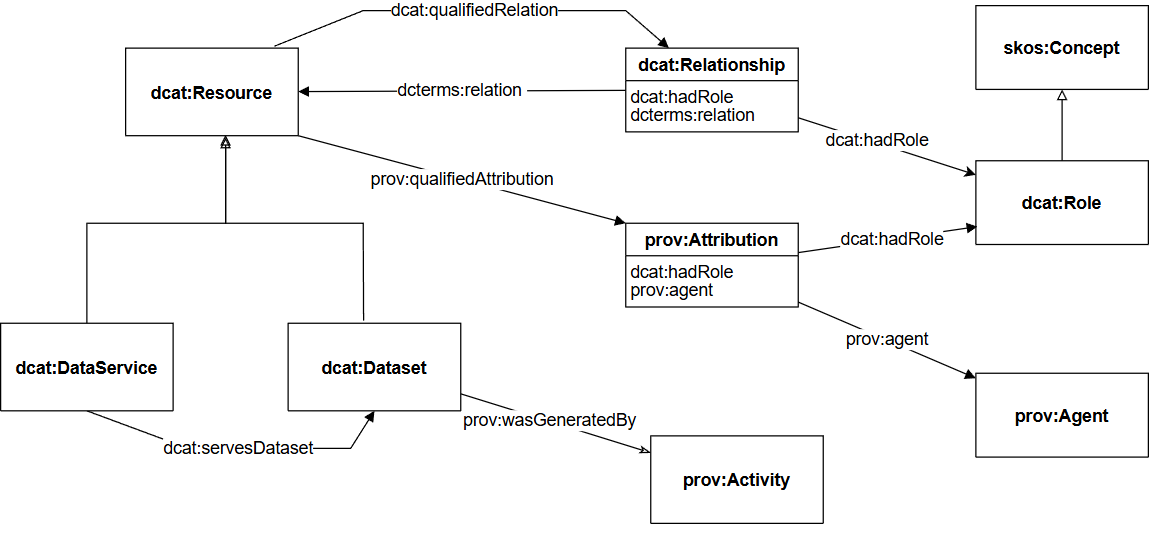
\includegraphics[width=1\textwidth]{figures/dcat.png}
    \caption{DCAT standard - prikazuje osnovne klase i svojstva za opisivanje kataloga podataka~\cite{dcat2020}}
    \label{fig:dcat_standard}
\end{figure}